\chapter{Methodology}
\label{chap:methodology}

\section{Architecture}
\label{sec:architecture}

\begin{figure}[H]
    \centering
    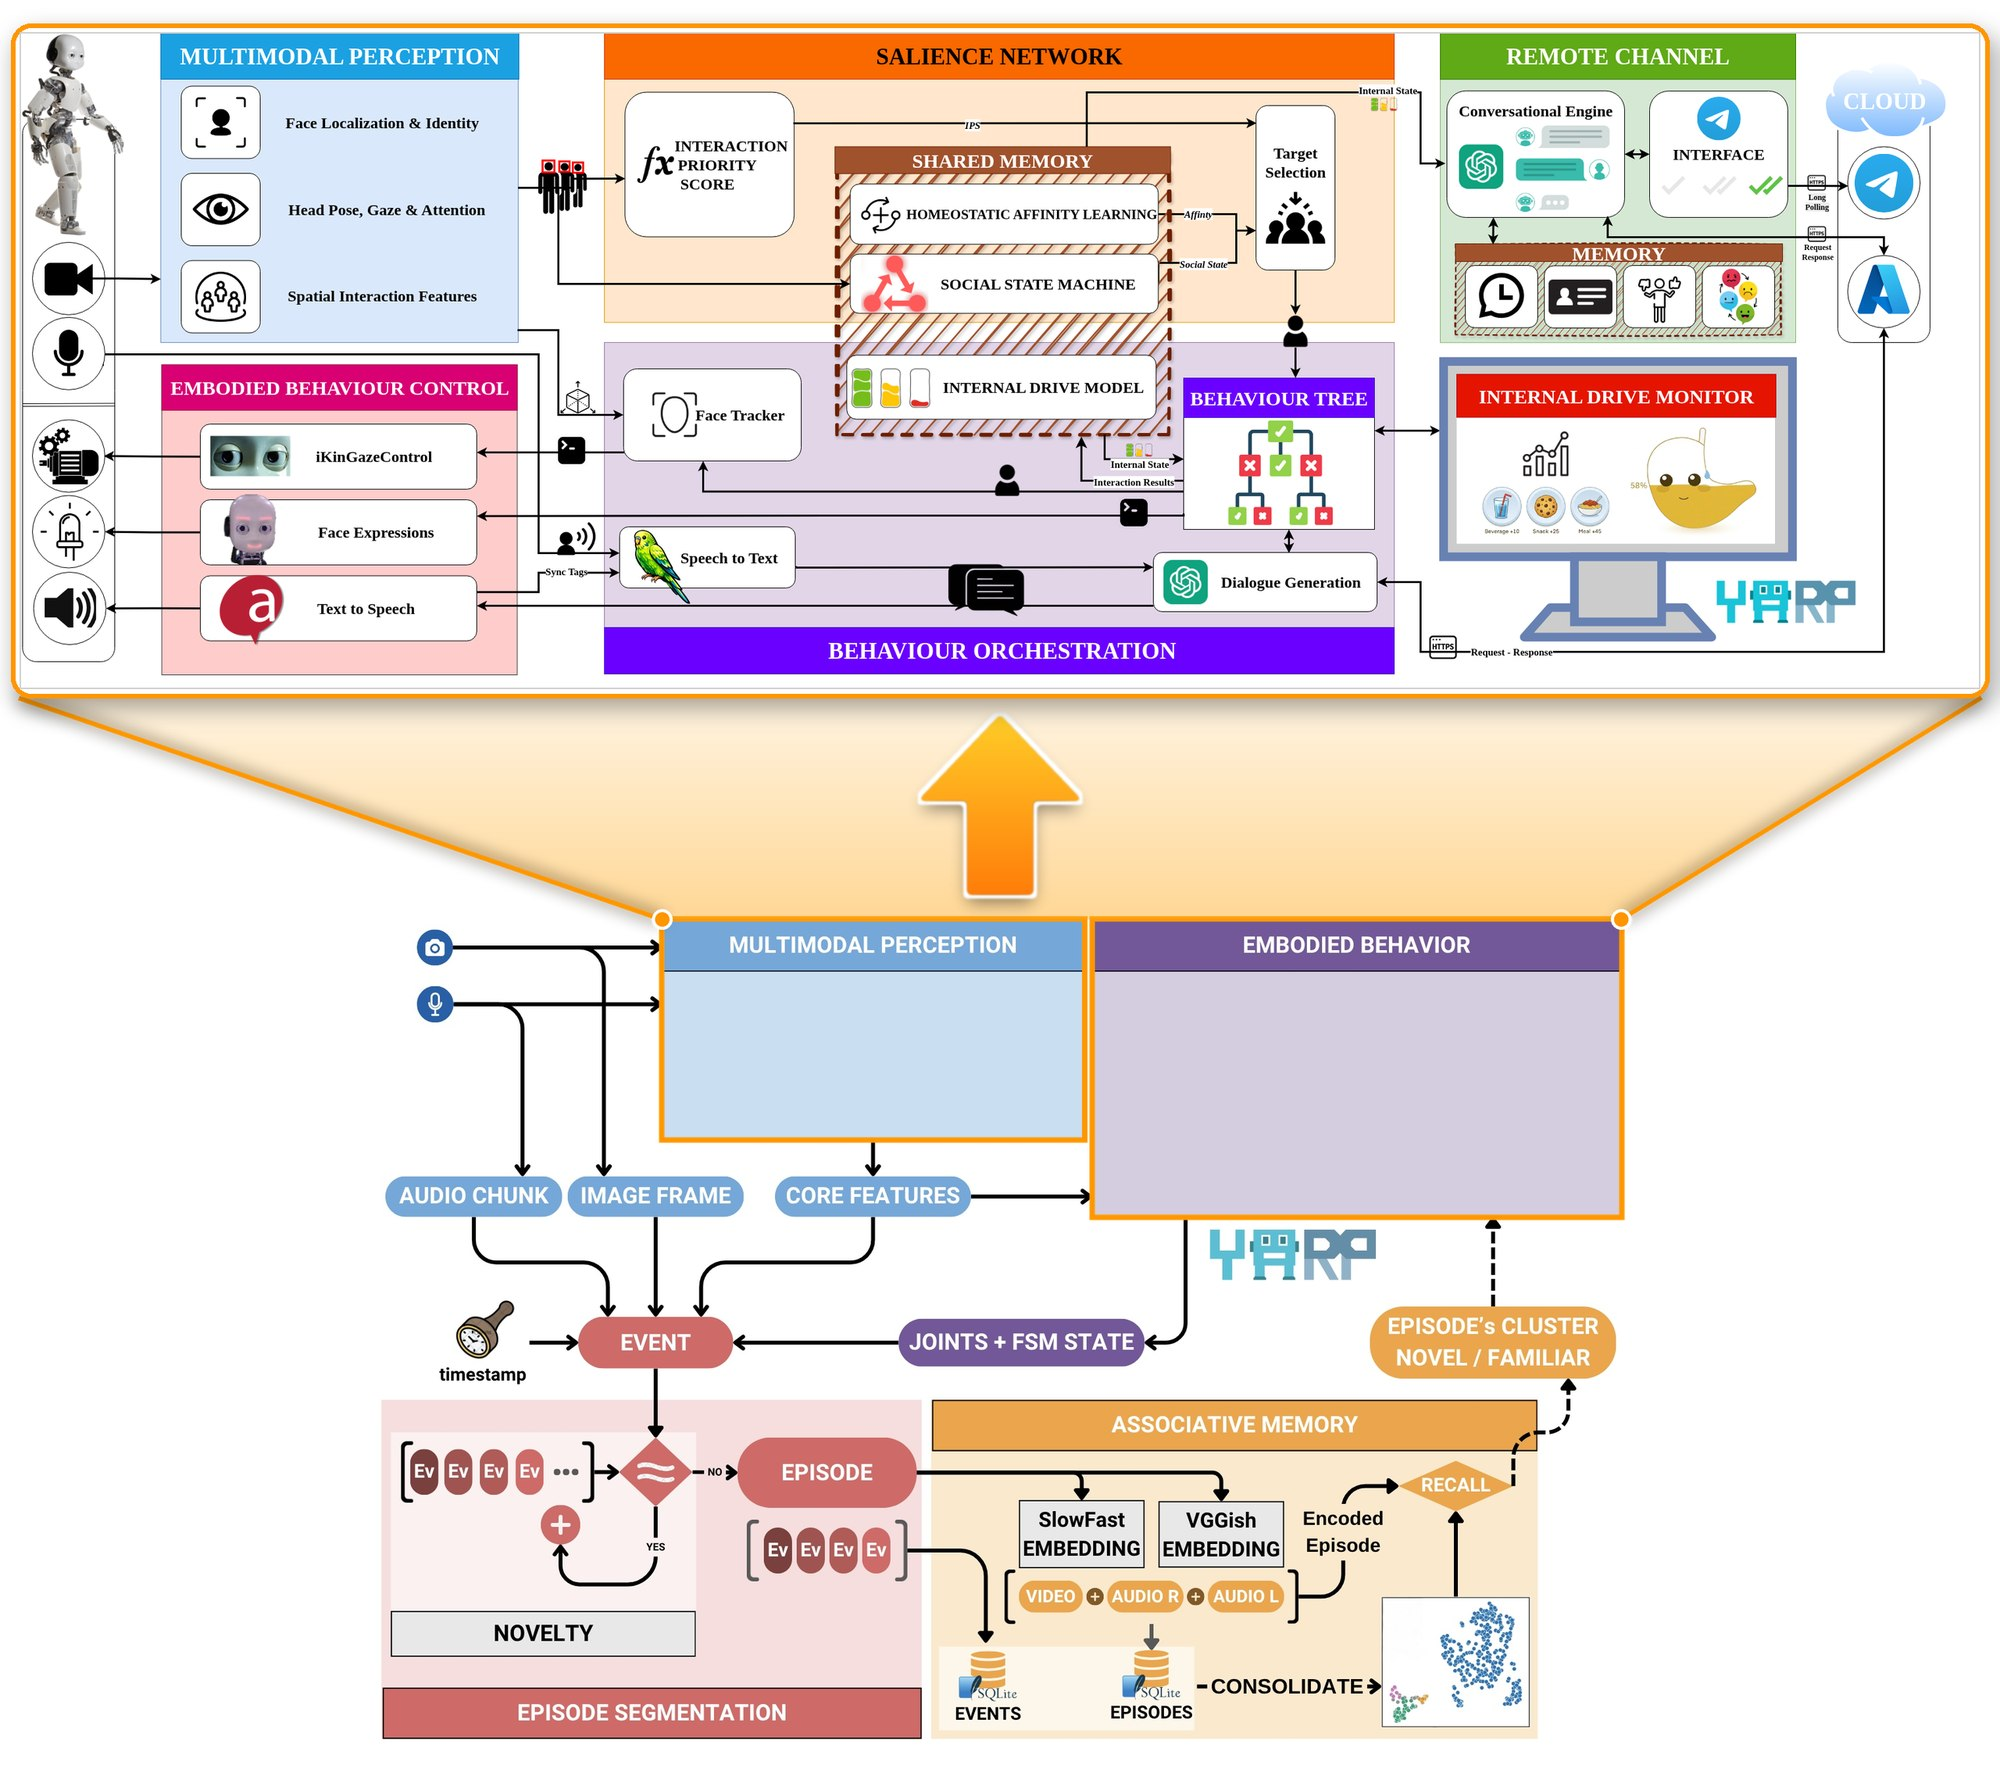
\includegraphics[width=\textwidth,height=0.48\textheight,keepaspectratio]{Methodology/Figures/always-on-with-embodied-behaviour.png}
    \caption[The embodied behaviour architecture within the always-on architecture.]{Place of this thesis in the always-on cognitive architecture of \citet{Pasquali2025AlwaysOn}. The magnified view (top) expands the Multimodal Perception and Embodied Behavior modules (bottom) into the embodied behaviour architecture developed here. Episode segmentation and associative memory are inherited.}
    \label{fig:always-on-embodied-overview}
\end{figure}

\subsection{Design rationale}
\label{subsec:architecture-rationale}

The \emph{Embodied Behaviour Architecture} developed in this thesis replaces the exploratory \emph{Embodied Behavior} module of the always-on cognitive architecture \citep{Pasquali2024ArtificialCognition,Pasquali2025AlwaysOn}, which had neither a value system nor action selection (Section~\ref{sec:intro-embodied-behaviour-architecture}). The new architecture splits embodied behaviour into four coordinated layers: salience-based attentional arbitration, executive dialogue gated by social state and drive, homeostatic self-regulation, and asynchronous remote outreach. Figure~\ref{fig:overall-architecture} shows the complete system.

Three things stay continuous across the layers. Each person keeps one track as they move. The robot's social and regulatory history with that person persists across sessions. The energy resource persists too, draining over time and by a fixed cost per social action. Two coupled loops build on this continuity. A 20~Hz sensorimotor loop turns the visual stream into fixation targets for the eyes and neck. A slower social and regulatory loop checks the deficit, starts proactive or reactive interactions, runs dialogue suited to the robot's state and updates social memory. The outcome of each interaction is credited to the person involved and sets the affinity that governs that person's later eligibility.

The organisation follows the open-system design of iCub, in which distributed perceptual and motor modules communicate through explicit middleware interfaces instead of one monolithic controller \citep{Metta2010ICub,Fischer2018ICubHRI}. It also follows a socially embedded model of autonomy, in which people are regulatory partners whose significance to the robot develops through repeated interaction \citep{Dautenhahn2002SociallyEmbedded}. Because executive control and homeostatic regulation meet only at these interfaces, conversational policies and drive models can be developed independently.

In the configuration evaluated here, the synthetic orexigenic deficit is the value signal. An event counts as positive if it reduces the deficit and negative if it increases it.

\begin{figure}[tbp]
    \centering
    \makebox[\textwidth][c]{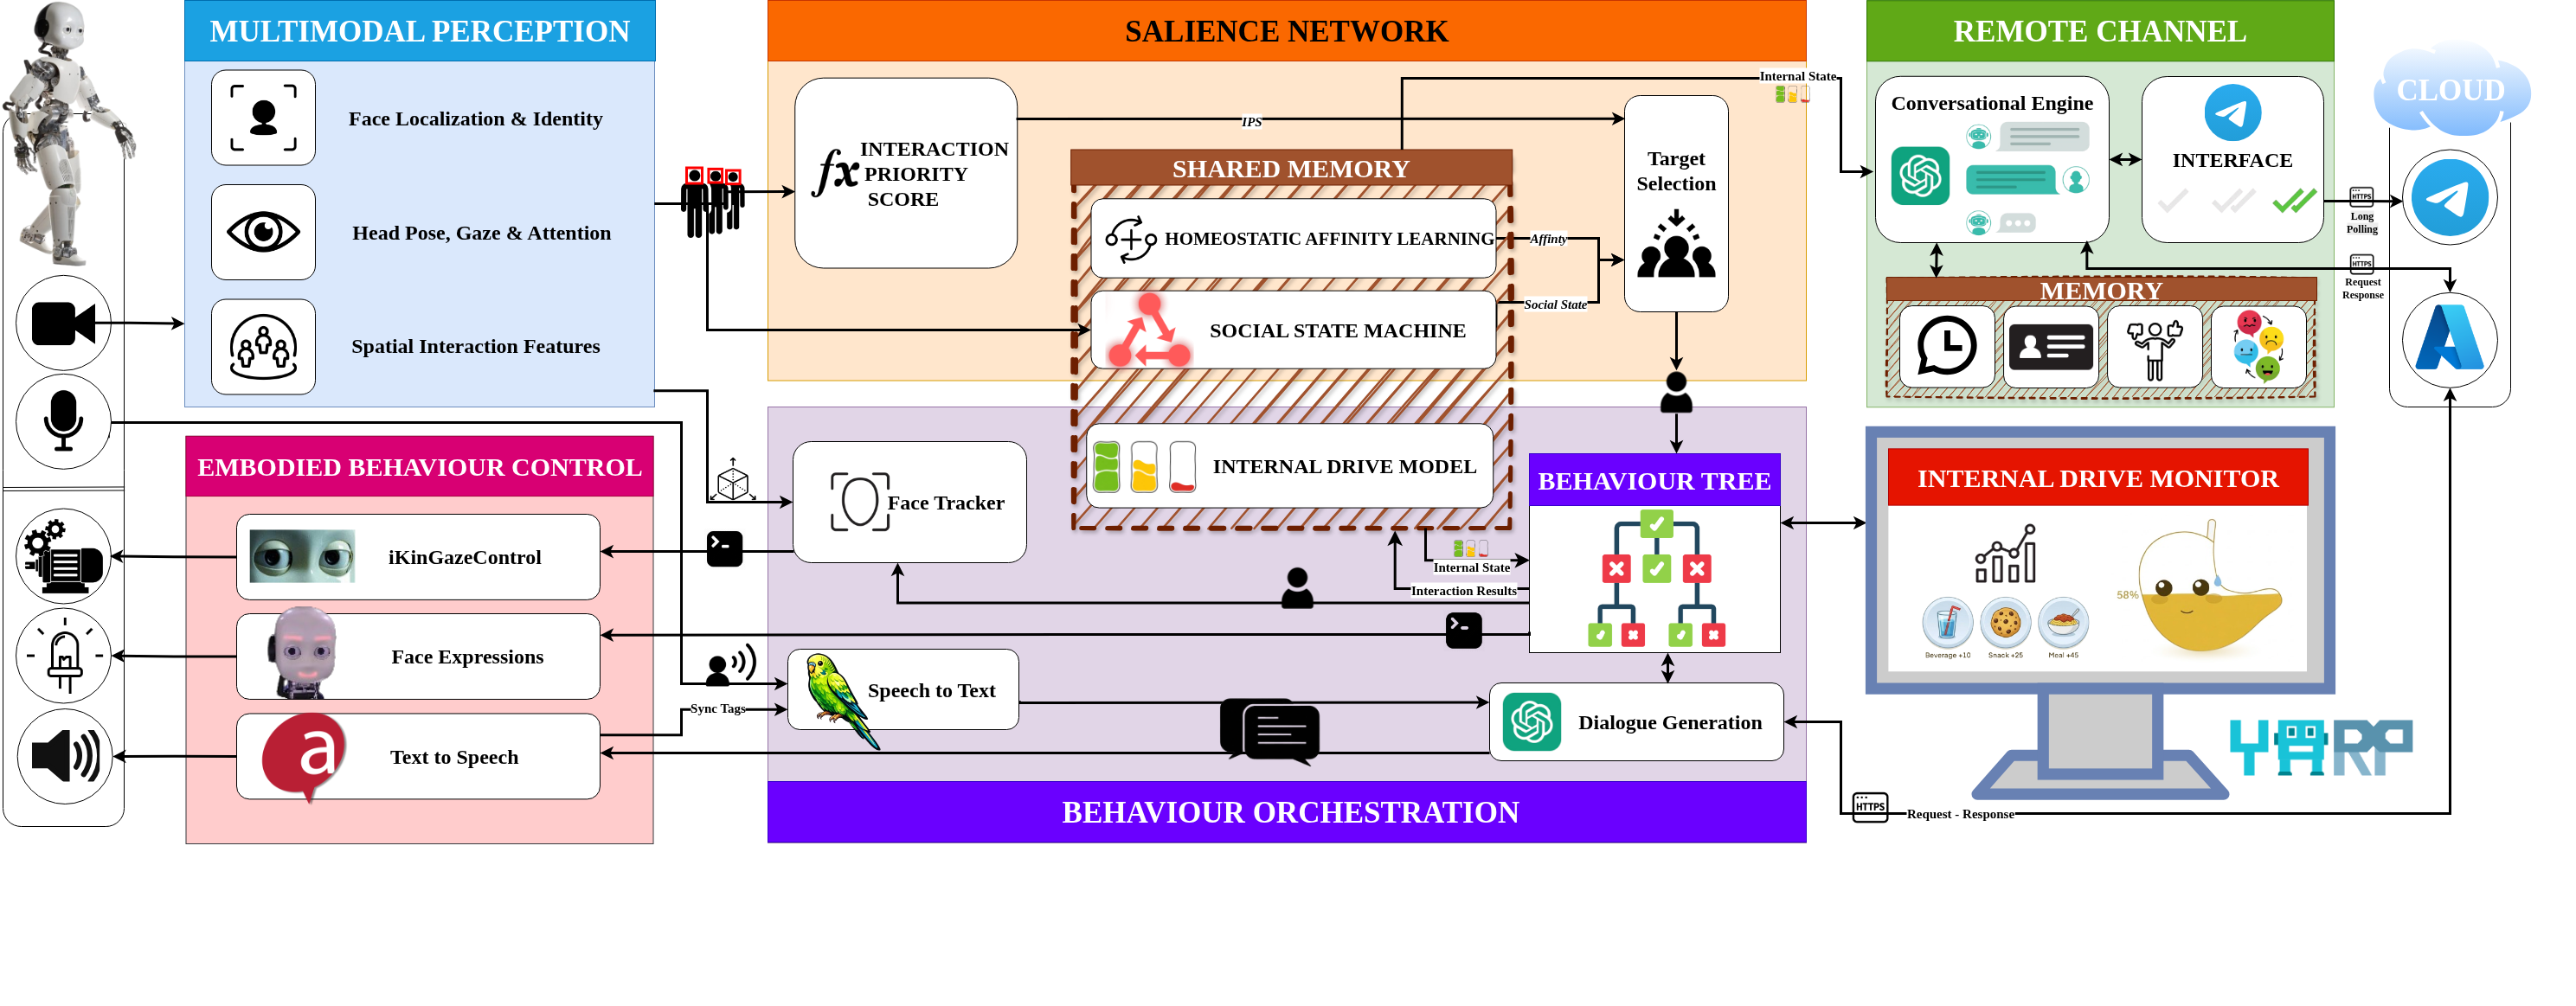
\includegraphics[width=\dimexpr\paperwidth-16mm\relax,height=0.5\textheight,keepaspectratio]{Methodology/Figures/overall-architecture.png}}
    \caption[Overall system architecture.]{Overall architecture of the always-on embodied behaviour system, showing perception, attentional selection, executive control, internal regulation, embodied output and the remote interaction channel.}
    \label{fig:overall-architecture}
\end{figure}

\subsection{Functional organisation}
\label{subsec:functional-organisation}

The system is an asynchronous network of modular services that communicate through YARP streaming ports and Remote Procedure Calls (RPCs) \citep{Metta2006YARP}. Camera frames, face records, speech events, drive telemetry, and meal payloads travel over streaming channels; RPCs handle one-off transitions such as starting an interaction, locking gaze, and enrolling an identity. Persistent drive, social, and experimental state is written atomically to JSON and SQLite stores.

Nominal update rates were 20~Hz for perception and attentional arbitration, 12.5~Hz for embodied gaze, 50~Hz for executive-state publication, 10~Hz for remote-state processing, and 30~Hz for the Internal Drive Monitor, the touchscreen that displays the drive and also accepts meals (Figure~\ref{fig:experimental-setup}). These are scheduler targets; actual throughput was limited by camera inference, message arrival and blocking input reads. Speech recognition ran per utterance, outside these fixed schedules. Table~\ref{tab:functional-layers} lists what each layer does.

\begin{table}[tbp]
    \centering
    \small
    \ra{1.2}
    \caption{Principal functional layers of the embodied behaviour architecture.}
    \label{tab:functional-layers}
    \begin{tabular}{@{}>{\raggedright\arraybackslash}p{0.16\textwidth}>{\raggedright\arraybackslash}p{0.19\textwidth}>{\raggedright\arraybackslash}p{0.29\textwidth}>{\raggedright\arraybackslash}p{0.23\textwidth}@{}}
        \toprule
\textbf{Layer} & \textbf{Primary input} & \textbf{Core transformation} & \textbf{Primary output} \\
\midrule
Multimodal Perception & Camera frames and microphone audio & Face detection, identity tracking, pose and gaze estimation, speech transcription & Per-person observations, scene features and utterance events \\
Always-On Context Memory & Continuous audiovisual stream and segmented episodes & VideoMAE and VGGish encoding, online UMAP/HDBSCAN recognition and neocortical consolidation & Context label and persistent episode memory \\
Salience Network & Per-person observations, social memory and context & Salience computation, eligibility gating and target arbitration & Gaze target and proactive interaction request \\
Behaviour Orchestration & Selected person, speech, internal state and meal events & Social-state-conditioned behaviour and dialogue orchestration & Speech, facial expression, memory updates and interaction outcome \\
Internal Drive Model & Time, action costs and feeding & Continuous depletion, categorical hunger state and regulatory reward & Internal state supplied to physical and remote behaviour \\
Remote Channel & Internal state, learned affinity and Telegram messages & Drive-conditioned dialogue and recipient selection & Asynchronous social contact and requests for human assistance \\
        \bottomrule
    \end{tabular}
\end{table}

The architecture separates the \emph{attention target} from the \emph{interaction target}. The robot often tracks the most salient person in the room without speaking to them. The executive controller starts an interaction only when that person clears an eligibility threshold, set by social state and learned affinity, and the context-dependent cooldown has elapsed. The separation mirrors the distinction between attention and confirmed engagement drawn by \citet{AbadMoya2026Initiation}, and it keeps exploratory gaze shifts from turning into unsolicited conversations.

\subsection{Coupling to always-on context memory}
\label{subsec:developmental-context-coupling}

The embodied architecture runs alongside the refactored, online version of the always-on cognitive architecture \citep{Pasquali2025AlwaysOn}, which assigns contexts online (Table~\ref{tab:functional-layers} and Section~\ref{subsec:intro-ecological-validation}). The salience module reads this streaming context label $\ell_t \in \{-1, 0, 1\}$ to set how often the robot initiates interaction: the lively context (label 1) shortens the cooldown between approaches, the calm context (label 0) lengthens it, and unclassified noise (label $-1$) applies a default (Equation~\ref{eq:context-cooldown}). Context thus changes how often the robot reaches out, without altering any person's perceptual score or affinity.

\section{Multimodal perception and person-centred scene representation}
\label{sec:multimodal-perception}

\subsection{Perceptual objective}
\label{subsec:perceptual-objective}

Social interaction requires a scene representation organised around people, in which location, presence over time, head orientation and readiness to communicate are tied to specific individuals. The baseline \emph{Multimodal Perception} module \citep{Pasquali2024ArtificialCognition,Pasquali2025AlwaysOn} tracked five aggregate features that did not distinguish between individuals (Section~\ref{subsec:intro-modular-organization}). With everyone present reduced to an anonymous count, a robot cannot ask a particular person for food, address a specific interlocutor or accumulate affinity toward anyone.

The vision module was therefore rewritten around individual people. It still computes the scene-level features and publishes them on the port the always-on memory reads, so episode segmentation receives the same features through the same interface as before. The gaze policy does differ: with no one in view the head now holds its last fixation instead of wandering, so the camera no longer sweeps the room and the scene those features describe changes accordingly. It processes $640\times480$ RGB frames and, when subscribers are connected, publishes one structured record per face on \texttt{landmarks:o}. Faces are detected in-process instead of being counted from a separate object-recognition module, then tracked and identified over time. Head pose, which the original module reduced to a count of people facing the camera, stays attached to each face. Appendix~\ref{app:vision-schema} lists the published schema.

\begin{figure}[tbp]
    \centering
    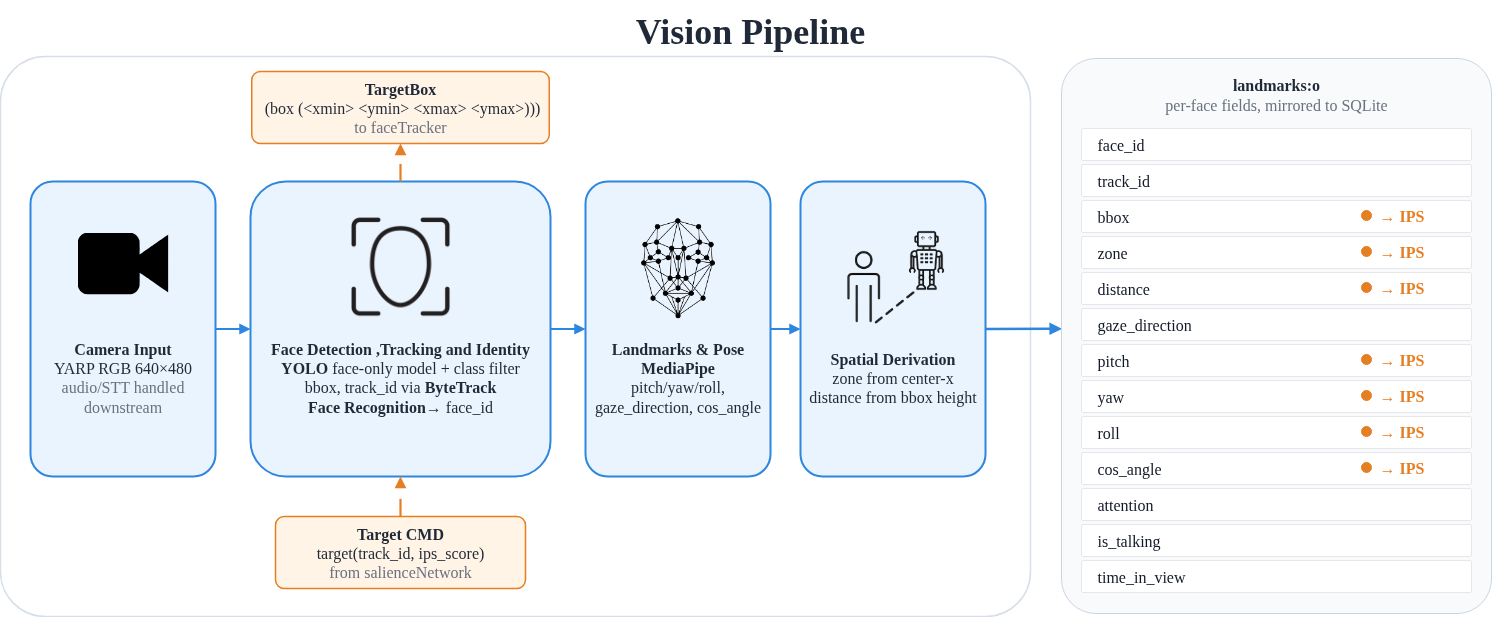
\includegraphics[width=0.88\textwidth,height=0.38\textheight,keepaspectratio]{Methodology/Figures/perception-pipeline.png}
    \caption[Vision-module processing and output pipeline.]{Vision-module pipeline from YARP camera input through YOLO/ByteTrack identity tracking and MediaPipe pose estimation to per-face \texttt{landmarks:o} records and the selected target-box output.}
    \label{fig:multimodal-perception-pipeline}
\end{figure}

\subsection{Face localisation, tracking and identity}
\label{subsec:face-tracking-identity}

Faces are found by the nano variant of the YOLO11 detector (YOLO11n) trained for faces, with a confidence threshold of $0.70$, and each box is expanded by 10\% per side. ByteTrack \citep{Zhang2022ByteTrack} tracks the boxes across frames and keeps a track alive through up to 120 processed frames of occlusion, 6~s at the nominal rate and about 20~s at the rate measured during deployment (Section~\ref{sec:results-operations}). For bounding box $\mathbf{b}_i=(x_i,y_i,w_i,h_i)$ in a $W\times H$ image, the normalised centre $(c_{x,i}/W, c_{y,i}/H)$ and relative face height $h_i/H$ describe position and apparent proximity independently of resolution; the zone thresholds in Table~\ref{tab:perception-gaze-parameters} bin them into five horizontal positions and four proximity classes.

Identity recognition matches 128-dimensional dlib facial embeddings against an enrolled gallery using combined minimum and median Euclidean distances. To suppress momentary misclassifications, a recognised name stays on its track through brief match failures, and a track still unknown is re-checked a limited number of times (Table~\ref{tab:perception-gaze-parameters}). When a person tells the robot their name, the vision module saves one face crop under that name, overwriting any earlier one, and keeps at most five prototype embeddings in memory; after a restart, one embedding is rebuilt from the stored crop.

\begin{table}[tbp]
    \centering
    \small
    \caption{Perception, identity and embodied gaze parameters.}
    \label{tab:perception-gaze-parameters}
    \begin{tabular}{@{}ll@{}}
        \toprule
        \textbf{Parameter} & \textbf{Value} \\
        \midrule
        Horizontal zone thresholds ($c_{x,i}/W$) & 0.20, 0.40, 0.60, 0.80 \\
        Proximity zone thresholds ($h_i/H$) & 0.10, 0.20, 0.40 \\
        Identity distance tolerance & 0.62 \\
        Identity track retention & 1.5 s \\
        Identity re-evaluation interval & 2.5 s \\
        Max identity retries & 3 \\
        Trajectory duration (eye, neck) & 0.6 s \\
        Reflex gains (vestibulo-ocular, oculo-collic) & 1.3, 0.8 \\
        \bottomrule
    \end{tabular}
\end{table}

\subsection{Head pose and gaze alignment}
\label{subsec:head-pose-gaze}

MediaPipe Face Landmarker extracts 478 3D landmarks per face: the 468-point face mesh plus 10 iris points. Head rotation $\mathbf{R}$ and translation $\mathbf{t}$ are estimated by Perspective-$n$-Point (PnP) optimisation over six standard facial points (nose tip, chin, eye corners, mouth corners):

\begin{equation}
    \lambda_j
    \begin{bmatrix}
        u_j\\v_j\\1
    \end{bmatrix}
    =
    \mathbf{K}
    \begin{bmatrix}
        \mathbf{R} & \mathbf{t}
    \end{bmatrix}
    \begin{bmatrix}
        \mathbf{X}_j\\1
    \end{bmatrix}.
    \label{eq:pnp-relation}
\end{equation}

Gaze alignment is the cosine between the head-forward vector $\mathbf{f}_i$ and the camera's optical axis $\mathbf{z}_c$:

\begin{equation}
    g_i=\cos\theta_i=
    \frac{\mathbf{f}_i^{\mathsf T}\mathbf{z}_c}
    {\lVert\mathbf{f}_i\rVert\lVert\mathbf{z}_c\rVert}.
    \label{eq:gaze-alignment}
\end{equation}

The camera is not calibrated: the intrinsic matrix $\mathbf{K}$ is approximated with $f_x=f_y=W$ and principal point $(W/2,H/2)$, and lens distortion is set to zero. The resulting $g_i$ is a coarse proxy for whether the head faces the camera; it does not measure where the eyes look.

Alignments $g_i > 0.90$ count as mutual gaze, $0.70 < g_i \leq 0.90$ as near gaze, and lower values as averted gaze. MediaPipe landmarks are fused with YOLO bounding boxes through greedy one-to-one assignment on normalised centre distance, gated by centre containment and box overlap. A tracked face that MediaPipe misses is still published, with its orientation marked unknown.

\subsection{Auditory and regulatory event streams}
\label{subsec:auditory-regulatory-streams}

Speech is transcribed locally by the Parakeet TDT 0.6B model, run as a quantised ONNX network. Bookmark signals from the speech synthesiser mute microphone input while the robot speaks, so the robot never transcribes its own voice. Speech heard during a dialogue is attributed to the current interlocutor; a greeting heard outside any interaction starts a reactive interaction with the largest visible face. Meal messages from the feeding cards (Section~\ref{subsec:meal-detection-attribution}) or the Internal Drive Monitor touchscreen carry increments of 10, 25 or 45 points and reach executive control through the same input stream.

\section{Salience-based attention selection and embodied gaze control}
\label{sec:salience-attention}

\subsection{From perceptual availability to interaction priority}
\label{subsec:interaction-priority}

Where the original gaze controller treated every face as equally urgent, the salience module gives each tracked person $i$ an Interaction Priority Score (IPS) combining apparent proximity $p_i$, image centricity $c_i$ and rectified gaze alignment $a_i$:

\begin{align}
    p_i &= \min\left(1,\frac{h_i}{H}\right), \label{eq:ips-proximity}\\
    c_i &= \max\left(0, 1-\frac{\sqrt{(c_{x,i}-W/2)^2+(c_{y,i}-H/2)^2}}{\sqrt{(W/2)^2+(H/2)^2}}\right), \label{eq:ips-centricity}\\
    a_i &= \max(0,g_i). \label{eq:ips-gaze}
\end{align}

The unnormalised base priority is computed as:

\begin{equation}
    I_i^{0}=0.50p_i+0.15c_i+0.50a_i.
    \label{eq:ips-base-score}
\end{equation}

When several people compete, a habituation multiplier $H_i$ scales the score; it is 1 for everyone except the current target (Section~\ref{subsec:habituation-hysteresis}):

\begin{equation}
    I_i=H_i\,I_i^{0}.
    \label{eq:ips-effective-score}
\end{equation}

\begin{figure}[tbp]
    \centering
    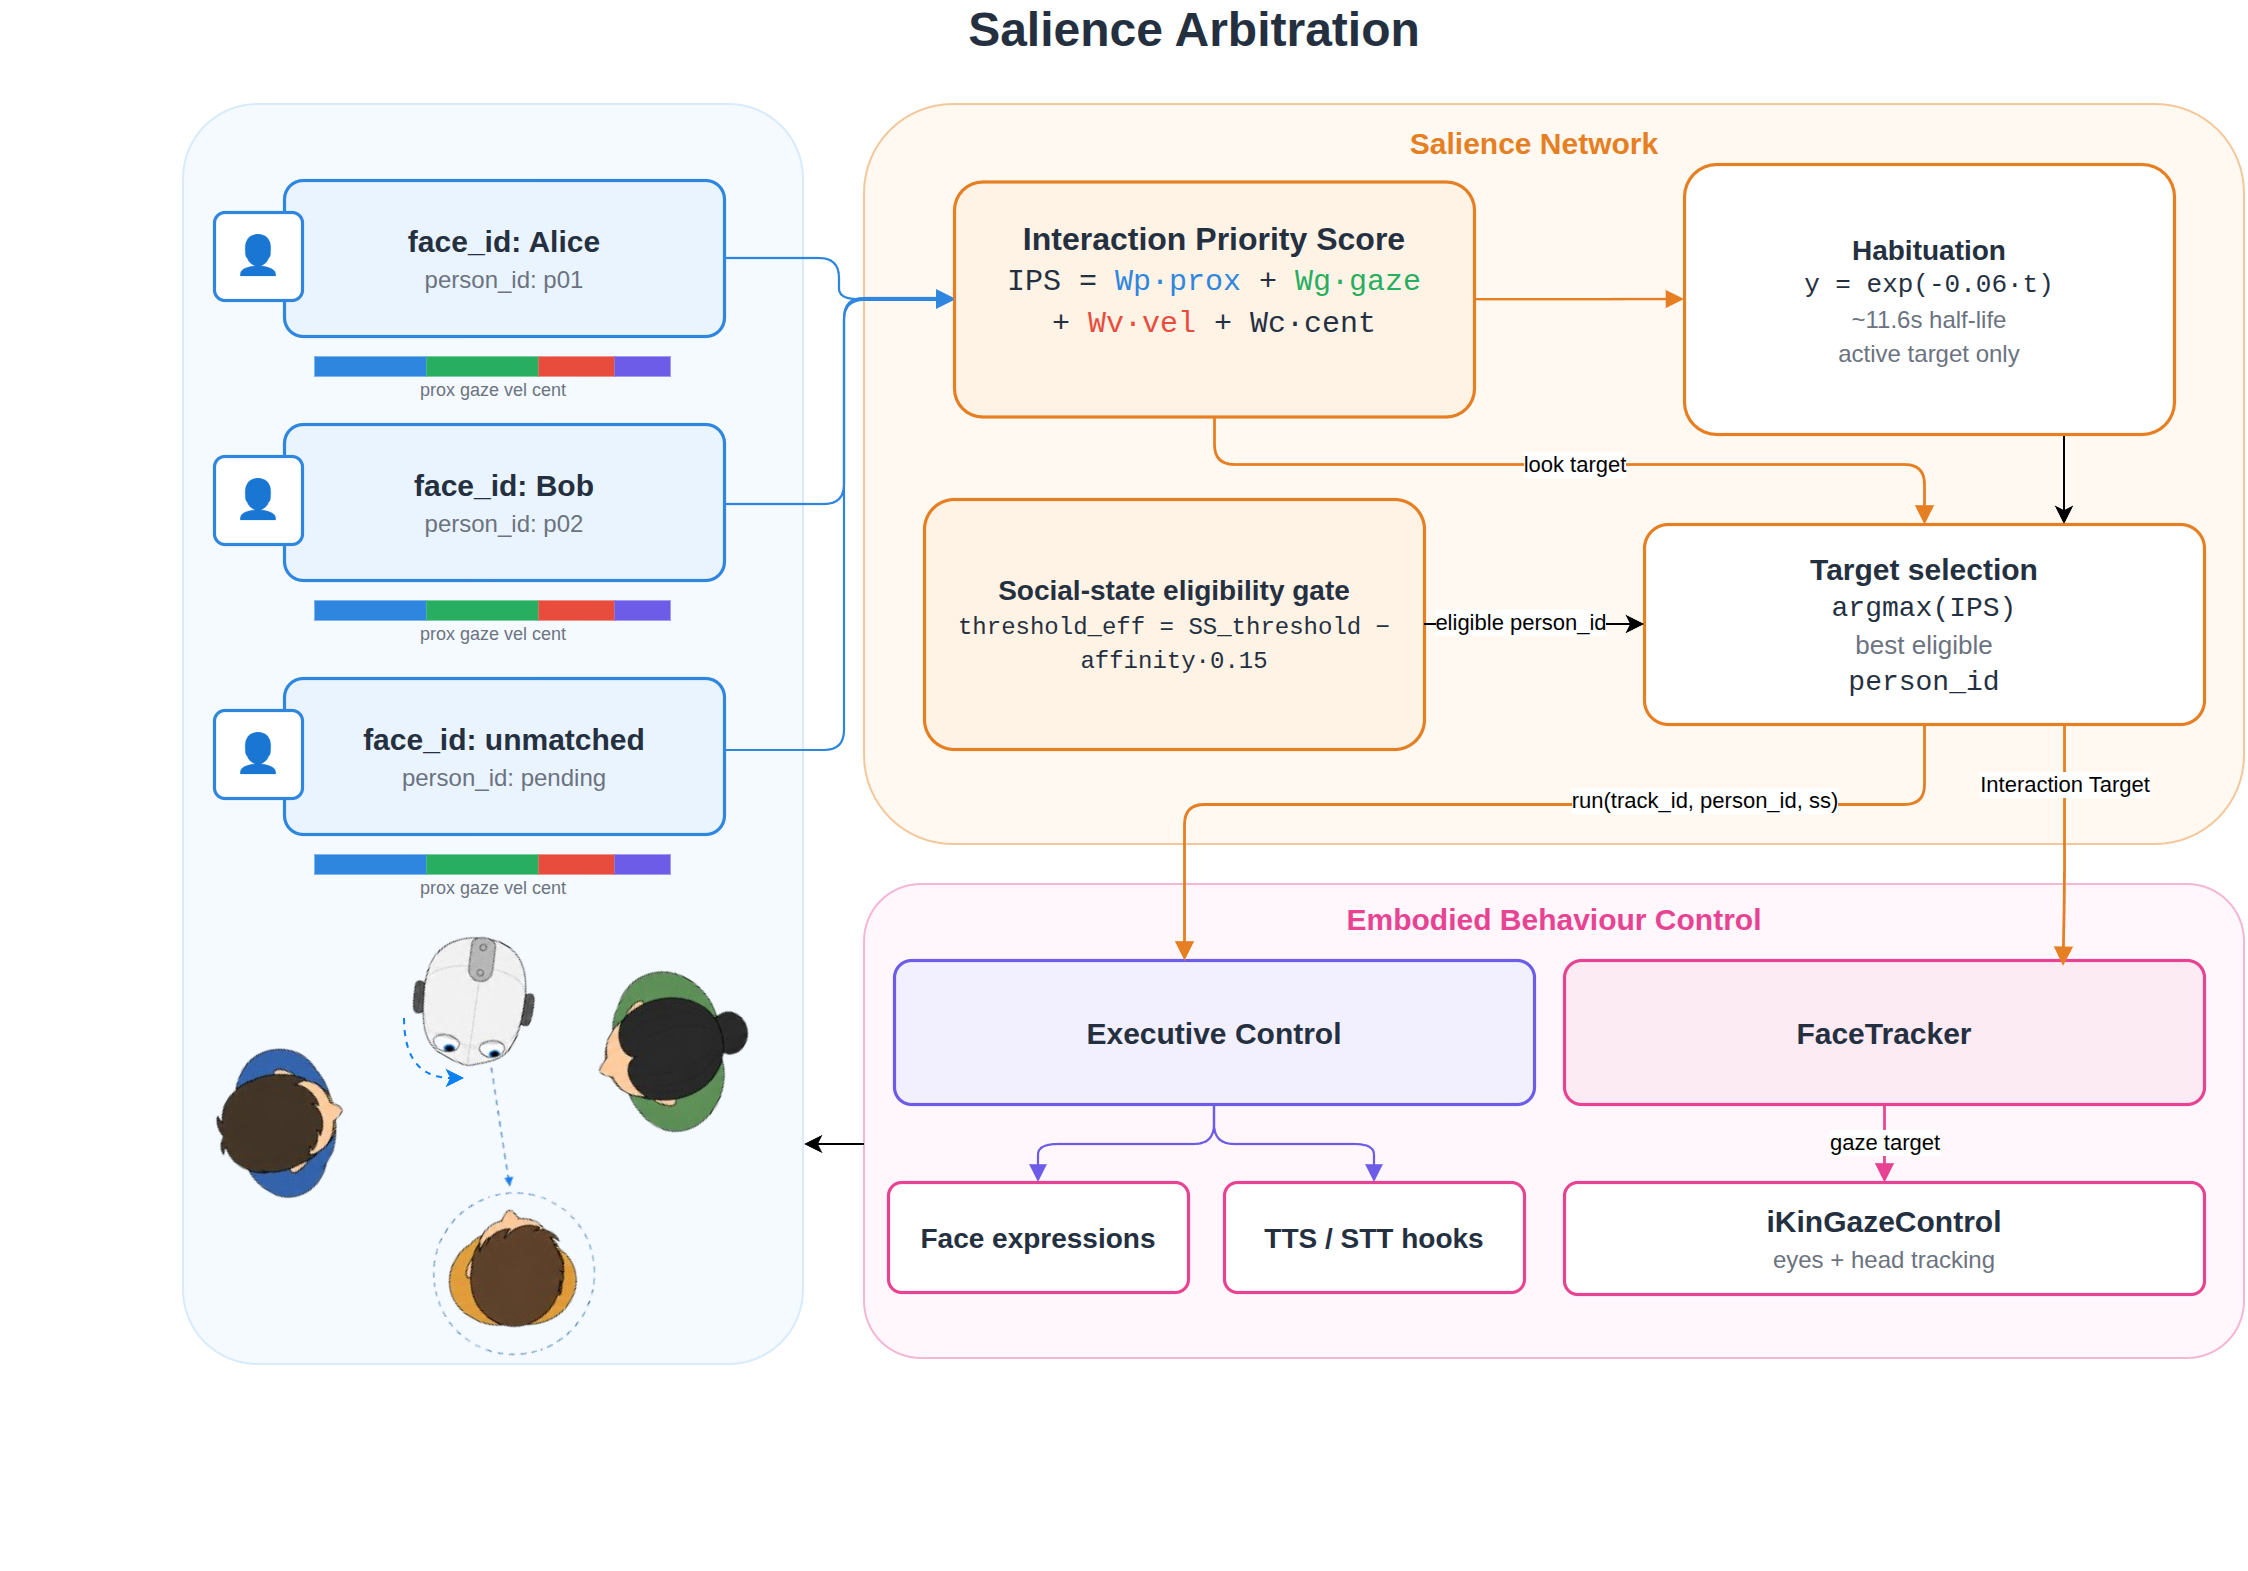
\includegraphics[width=0.88\textwidth,height=0.38\textheight,keepaspectratio]{Methodology/Figures/salience-arbitration.png}
    \caption[Salience arbitration.]{Salience arbitration from per-person perceptual features and social-memory gates to gaze selection and interaction initiation.}
    \label{fig:salience-arbitration}
\end{figure}

\subsection{Social-state and affinity-dependent eligibility}
\label{subsec:affinity-eligibility}

Personalisation leaves the perceptual weights unchanged and acts instead on the eligibility threshold $\theta_i$, which depends on social state $s_i$ (Section~\ref{subsec:social-state-history}) and learned homeostatic affinity $A_i \in [-1, 1]$:

\begin{equation}
    \theta_i=\max\left(0.50,\theta_{s_i}-0.15A_i\right),
    \label{eq:effective-interaction-threshold}
\end{equation}
\begin{equation}
    (\theta_{\mathrm{Unknown}},\theta_{\mathrm{Recognised}}, \theta_{\mathrm{Greeted}},\theta_{\mathrm{Engaged}}) = (0.80,0.65,0.70,0.85).
    \label{eq:social-state-thresholds}
\end{equation}

A person is eligible for proactive engagement when $I_i \geq \theta_i$; if the identity is still unresolved, the request waits up to 5~s for recognition to settle. Positive affinity lowers the threshold by up to 0.15, so the robot more readily approaches people who have fed it, and negative affinity raises it by as much. Repeated approaches are spaced by the context cooldown $T_{\mathrm{cd}}(\ell_t)$:

\begin{equation}
    T_{\mathrm{cd}}(\ell_t)=
    \begin{cases}
        3~\mathrm{s}, & \ell_t=1 \quad \text{(lively)},\\
        15~\mathrm{s}, & \ell_t=0 \quad \text{(calm)},\\
        5~\mathrm{s}, & \ell_t=-1 \quad \text{(fallback or noise)}.
    \end{cases}
    \label{eq:context-cooldown}
\end{equation}

\subsection{Habituation, hysteresis and target stability}
\label{subsec:habituation-hysteresis}

To stop gaze from flipping between equally salient people, the current target's score decays exponentially while a competitor stays in view, with $\tau$ counted from the end of the 5~s dwell:

\begin{equation}
    H_i(\tau)=\exp(-\lambda\tau), \qquad \lambda=0.06\ \mathrm{s}^{-1}.
    \label{eq:habituation}
\end{equation}

Gaze switches from the current target $k$ to the challenger $j = \argmax_i I_i$ only if

\begin{equation}
    I_j > I_k + \delta \quad\land\quad t - t_{\mathrm{switch}} \geq T_{\mathrm{dwell}},
    \label{eq:switch-suppression}
\end{equation}

with hysteresis margin $\delta=0.10$ and minimum dwell $T_{\mathrm{dwell}}=5$~s. With no current target, gaze is assigned only when the highest score reaches 0.60. An active dialogue locks gaze to the interlocutor and overrides this arbitration.

\subsection{Embodied target execution}
\label{subsec:embodied-target-execution}

The selected track is streamed to the vision module, which resolves its current box; the box centre is projected through the iCub gaze controller iKin\-Gaze\-Control to a 3D fixation point $\mathbf{p}_t$ at fixed depth $z_0=0.7$~m:

\begin{equation}
    \mathbf{u}_t=\begin{bmatrix} x_t+w_t/2\\y_t+h_t/2 \end{bmatrix}, \qquad \mathbf{p}_t=G_L(\mathbf{u}_t,z_0).
    \label{eq:facetracker-projection}
\end{equation}

A motor command is sent only when the target moves beyond a pixel deadband:

\begin{equation}
    \gamma_t = \mathbb{I}\!\left(|u_{x,t}-u_{x,t^-}|>8 \;\lor\; |u_{y,t}-u_{y,t^-}|>25\right).
    \label{eq:facetracker-deadband}
\end{equation}

The FaceTracker module that sends these commands projects through the left-camera model ($G_L$), enables continuous iKin tracking, fixes neck roll at zero, leaves neck pitch free and disables saccades. Without a valid target it sends no neutral-pose command, so the last fixation holds until a new one replaces it.

\section{Executive control: social-state orchestration and drive-gated behaviour logic}
\label{sec:executive-control}

\subsection{Interaction ownership and trigger modes}
\label{subsec:interaction-ownership}

Executive control coordinates dialogue, speech synthesis and facial expressions, and only one interaction can own these resources at a time. Proactive requests (triggered by salience) and reactive greetings (triggered by unsolicited speech) enter the same finite-state machine. Proactive entry requires the person to answer the robot's greeting before the interaction continues; reactive entry skips that step, since the person has already spoken, and shortens the greeting and name exchange. In the state machine (Figure~\ref{fig:executive-control-transitions}), every interaction first acquires ownership; only then does the branch that decides what is said take over.

\begin{figure}[tbp]
    \centering
    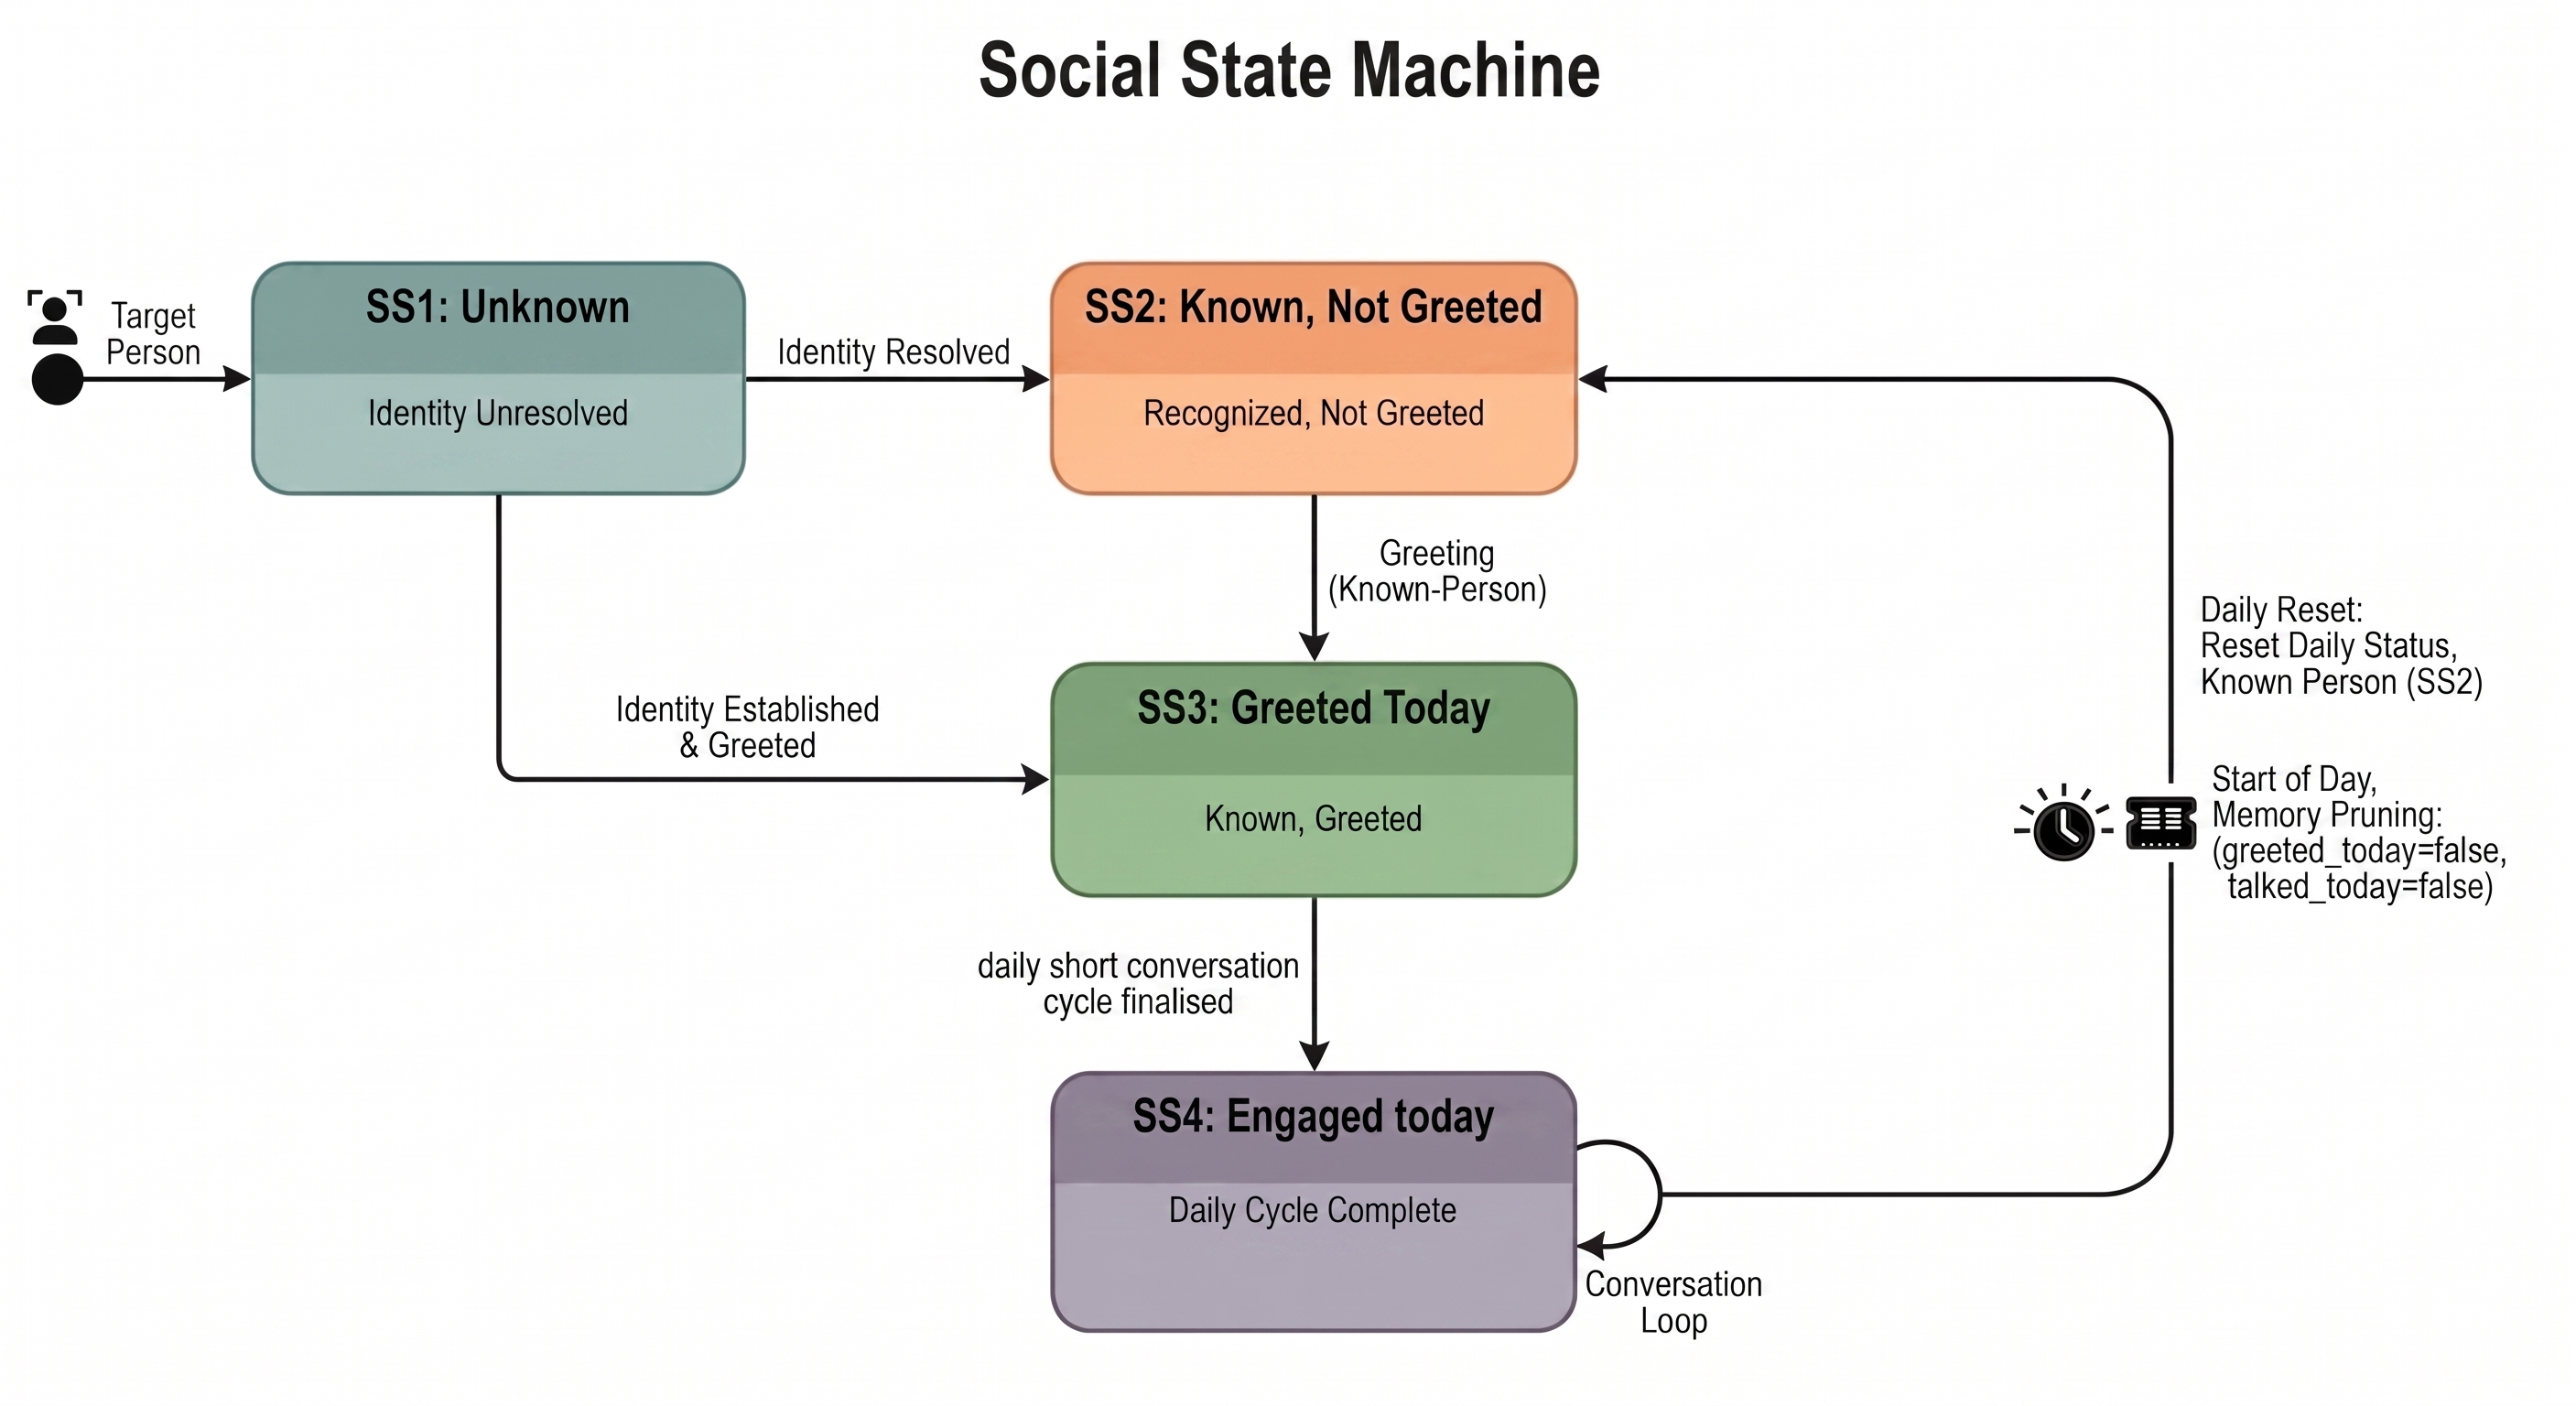
\includegraphics[width=0.88\textwidth,height=0.38\textheight,keepaspectratio]{Methodology/Figures/executive-state-transitions.png}
    \caption[Executive-control state transitions.]{Executive-control state transitions, showing proactive and reactive entry, social-state-conditioned behaviour, the Starving-state override, target monitoring and interaction completion.}
    \label{fig:executive-control-transitions}
\end{figure}

\subsection{Social state as interaction history}
\label{subsec:social-state-history}

Social history with person $i$ is described by three flags: whether the person is recognised ($K_i$), has been greeted today ($G_i$), and has completed at least one conversational turn today ($T_i$):

\begin{equation}
    s_i=
    \begin{cases}
        \mathrm{Unknown}, & \neg K_i,\\
        \mathrm{Recognised}, & K_i\land\neg G_i,\\
        \mathrm{Greeted}, & K_i\land G_i\land\neg T_i,\\
        \mathrm{Engaged}, & K_i\land G_i\land T_i.
    \end{cases}
    \label{eq:social-state-function}
\end{equation}

An Unknown person gets an introduction and is asked for their name, a Recognised person gets a greeting by name, and a Greeted person gets open conversation.

\subsection{Drive-gated behavioural policy}
\label{subsec:drive-gated-policy}

The hunger state $h \in \{\mathrm{Disabled}, \mathrm{Full}, \mathrm{Hungry}, \mathrm{Starving}\}$, where Disabled means the drive is switched off, decides which behaviour runs:

\begin{equation}
    \pi(s,h)=
    \begin{cases}
        \pi_{\mathrm{reg}}(s), & h=\mathrm{Starving},\\
        \pi_{\mathrm{Unknown}}, & h\neq\mathrm{Starving}\land s=\mathrm{Unknown},\\
        \pi_{\mathrm{Recognised}}, & h\neq\mathrm{Starving}\land s=\mathrm{Recognised},\\
        \pi_{\mathrm{Greeted}}, & h\neq\mathrm{Starving}\land s=\mathrm{Greeted},\\
        \pi_{\mathrm{Greeted}}, & h\neq\mathrm{Starving}\land s=\mathrm{Engaged}\land I_i\geq\theta_i,\\
        \pi_{\varnothing}, & \text{otherwise}.
    \end{cases}
    \label{eq:executive-policy}
\end{equation}

Algorithm~\ref{alg:executive-control} spells out the Starving branch, its timeouts and when conversation resumes. All other states share the social-state branches of Equation~\ref{eq:executive-policy}, and Hungry differs from Full only through hunger-state prompt overlays (Section~\ref{subsec:language-model-instantiation}). Hunger never enters the IPS or eligibility equations: the Starving branch sets executive priority only once an interaction has started. Remote escalation is specified separately in Section~\ref{subsec:stable-transitions}.

\begin{algorithm}[tbp]
\caption{Behaviour-tree-equivalent social-state and drive-gated executive control}
\label{alg:executive-control}
\small
\begin{algorithmic}[1]
    \STATE Receive either a proactive request or a reactive greeting event
    \IF{another interaction owns executive resources}
        \STATE Reject the new request
    \ENDIF
    \STATE Acquire interaction ownership and lock gaze to the selected person
    \STATE Record initial social state, internal state and resource level
    \STATE Start target-continuity monitoring
    \STATE \textbf{Priority selector:}
    \IF{critical depletion is active}
        \STATE Request feeding
        \STATE Wait 8~s for a valid meal; retry once, then fail on a second consecutive timeout
        \STATE Acknowledge each meal and test whether Full has been restored
        \STATE Continue until Full, target loss, drive disablement or timeout failure
        \IF{Full is restored and the interrupted branch was Greeted}
            \STATE Resume the conversational sequence
        \ENDIF
    \ELSE
        \IF{state is Unknown}
            \STATE Greet and require a response \COMMENT{reactive entry: skip the response requirement, the greeting already elicited one}
            \STATE Request and extract the name with one retry
            \STATE Enrol identity, acknowledge introduction and optionally continue to Greeted
        \ELSIF{state is Recognised}
            \STATE Greet by name with at most two attempts, update memory and enter Greeted \COMMENT{reactive entry: one attempt, shorter timeout}
        \ELSIF{state is Greeted}
            \STATE Generate a short opener
            \STATE Generate full replies for three turns, then brief acknowledgements
            \STATE Continue until silence, target loss or interruption
            \STATE Mark Engaged once at least one conversational turn is completed
        \ELSIF{state is Engaged and again eligible}
            \STATE Execute the Greeted conversational branch while retaining Engaged memory
        \ENDIF
    \ENDIF
    \STATE Record final resource level, energetic cost and behavioural outcome
    \STATE Release target and interaction ownership
    \STATE Return the compact outcome to attentional learning
\end{algorithmic}
\end{algorithm}

\subsection{Language-model instantiation}
\label{subsec:language-model-instantiation}

Embodied dialogue used Azure OpenAI GPT-4.1-mini, whereas Telegram dialogue used GPT-5-mini. Versioned templates in \texttt{prompts.json} supplied persona and hunger-state overlays (Appendix~\ref{app:prompts}). Embodied starter, reply, and wind-down budgets were 40, 56, and 18 completion tokens; the corresponding Telegram reply, proactive-message, and summary caps were 800, 800, and 900. Sampling temperature was left at the service default.

\section{Orexigenic homeostasis, homeostatic affinity learning, and adaptive social memory}
\label{sec:homeostasis-affinity-memory}

\subsection{Synthetic orexigenic drive}
\label{subsec:internal-regulation-model}

The synthetic orexigenic drive models an internal resource level $x(t) \in [0, 100]$, measured in stomach points (points hereafter). Without other input, $x$ decays linearly at the passive rate $\rho = 100/(4\times3600)$~points/s, emptying a full reserve in 4~h. Each social action costs a discrete amount $C_t$, and each meal adds an increment $M_t$:

\begin{equation}
    x_{t+\Delta t}=\operatorname{clip}_{[0,100]}\left(x_t-\rho\Delta t-C_t+M_t\right).
    \label{eq:resource-dynamics}
\end{equation}

While the drive is enabled, the continuous level maps onto three states:

\begin{equation}
    h(x)=
    \begin{cases}
        \mathrm{Full}, & x\geq60,\\
        \mathrm{Hungry}, & 25\leq x<60,\\
        \mathrm{Starving}, & x<25.
    \end{cases}
    \label{eq:regulatory-state-partition}
\end{equation}

Hungry lets the robot voice its need before the resource enters the critical Starving region, where feeding requests take priority over ordinary dialogue. Voicing need early is still not allostasis, which anticipates demand \citep{Sterling2012Allostasis,SchulkinSterling2019Allostasis}: this controller reads only the current level and forecasts neither depletion nor caregiver availability. The analogy with appetite is functional: stomach points and action costs measure neither metabolism nor real battery use. Figure~\ref{fig:orexigenic-dynamics} illustrates the resource dynamics. Action costs scale with verbal load: a greeting or a feeding acknowledgement costs 0.8 points, a name request or a feeding request 1.0, a conversation opener 1.2 and a full conversational turn 3.6.

\begin{figure}[tbp]
    \centering
    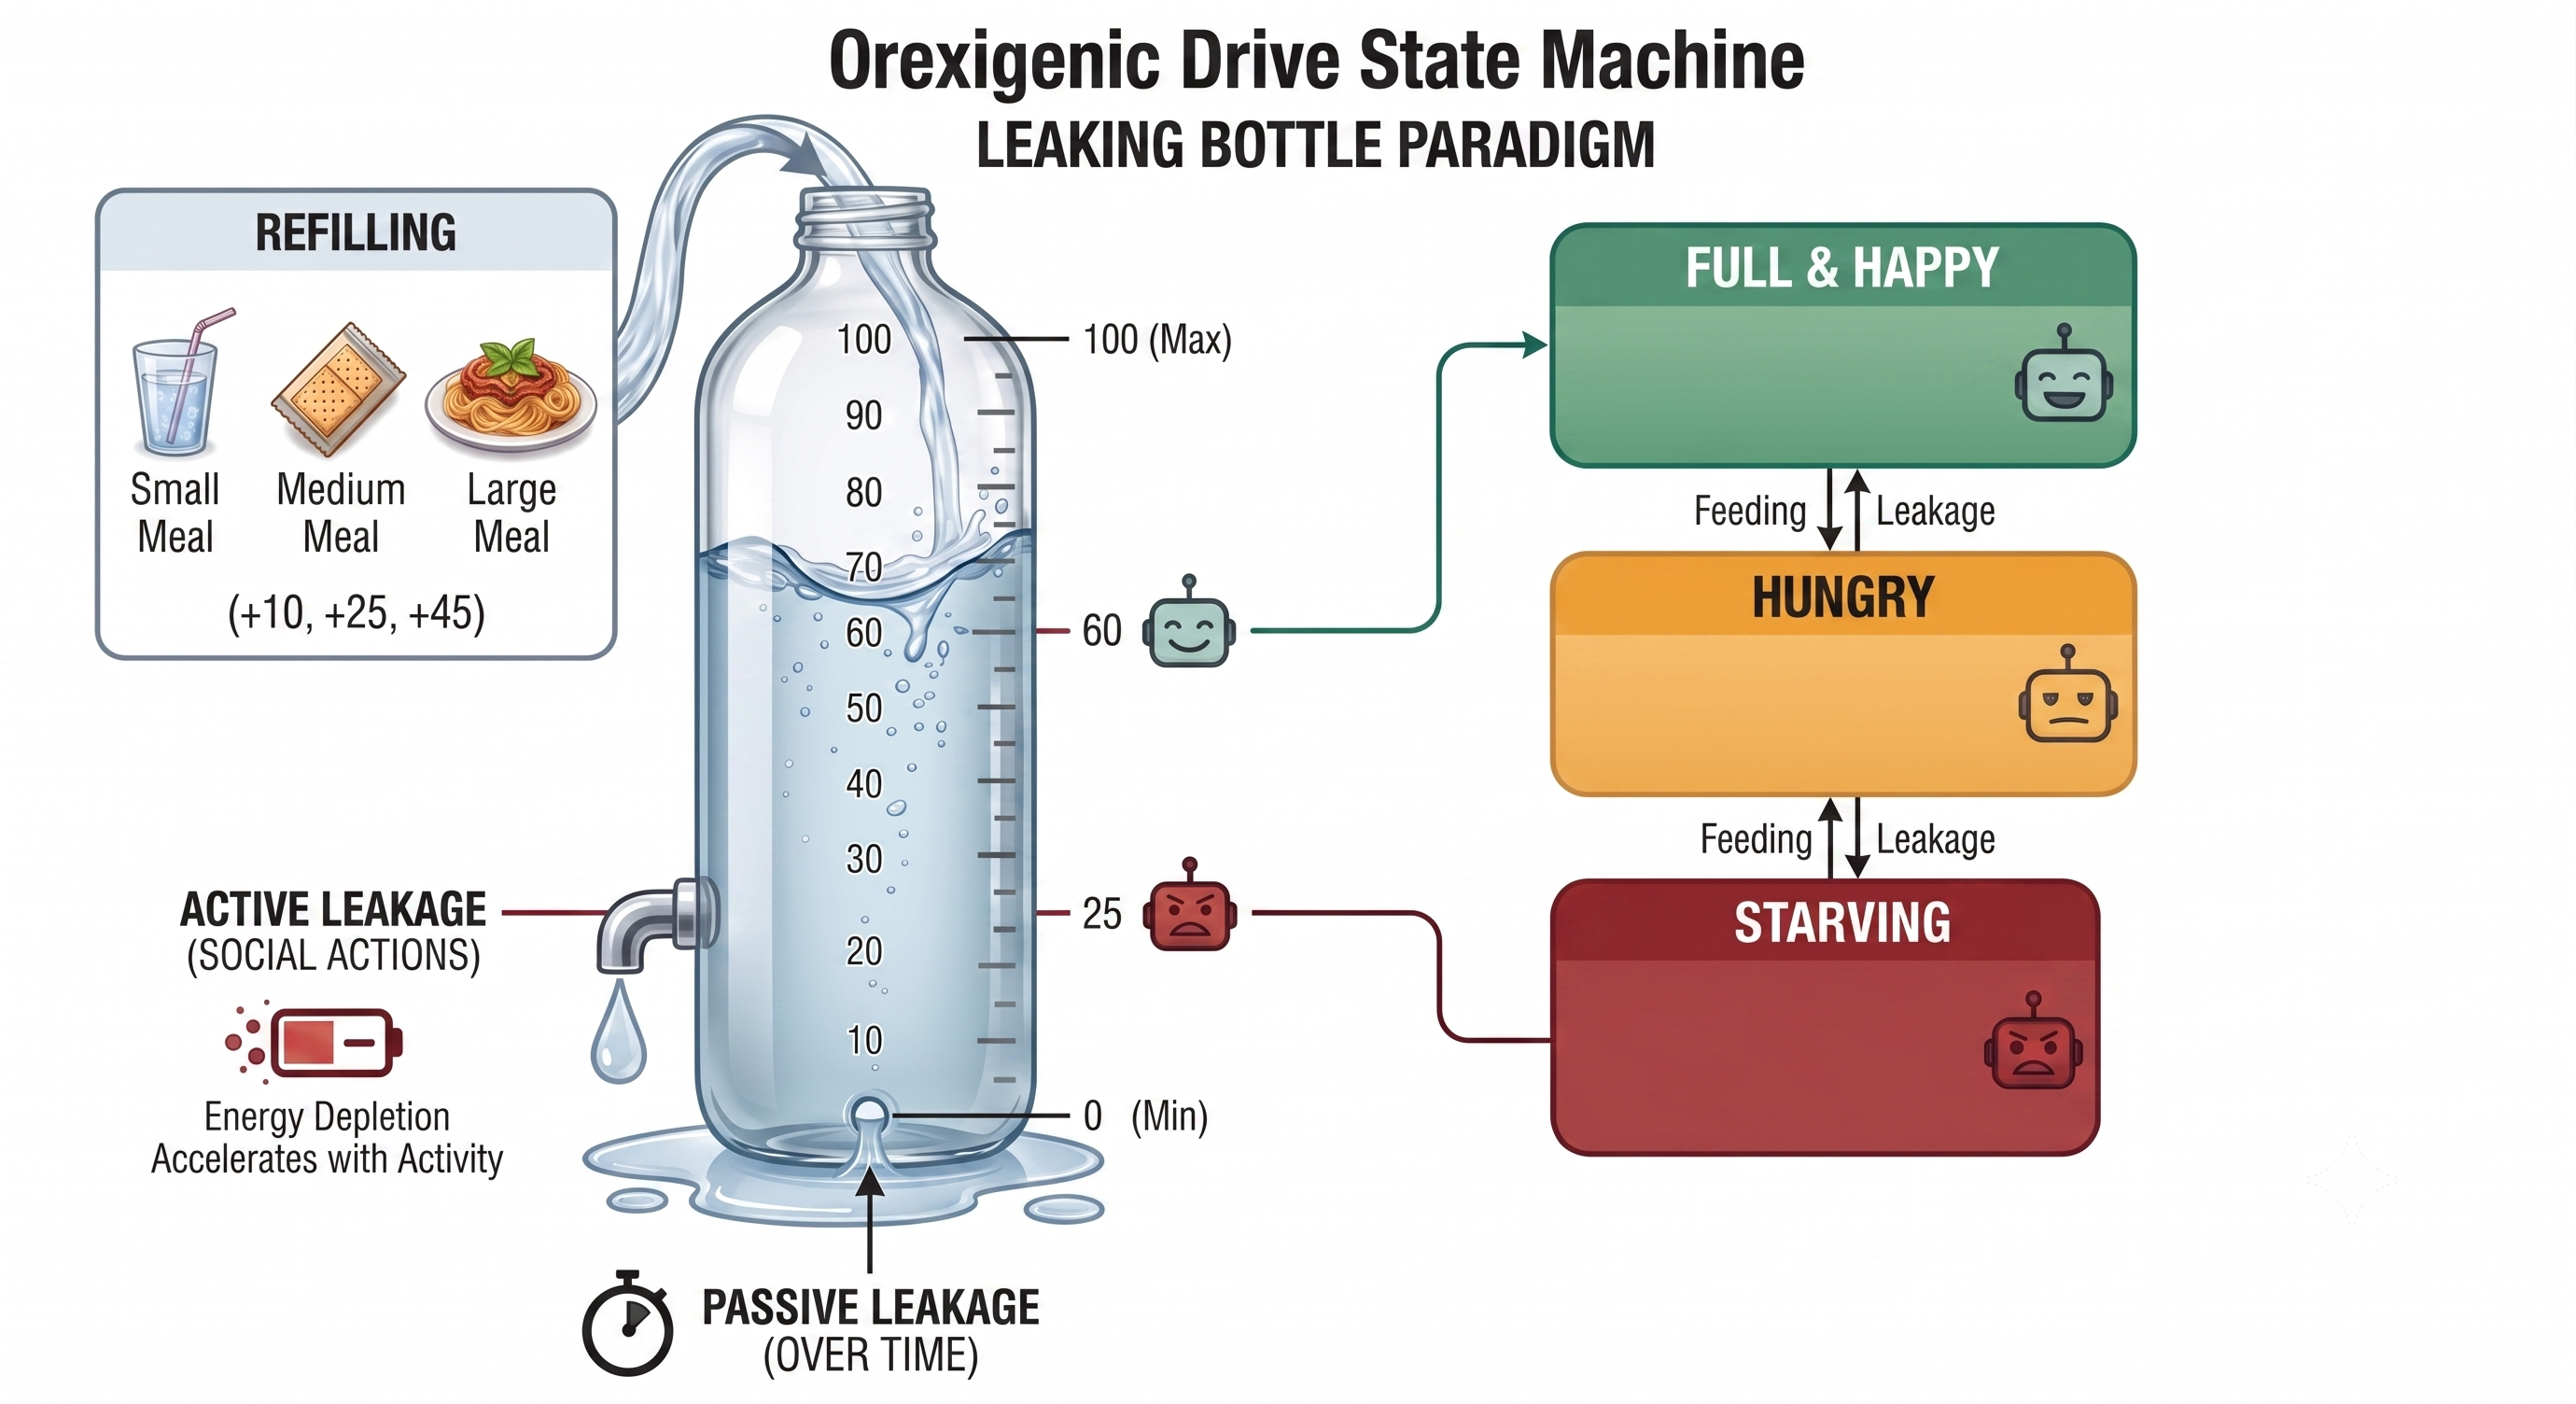
\includegraphics[width=0.88\textwidth,height=0.38\textheight,keepaspectratio]{Methodology/Figures/orexigenic-dynamics.png}
    \caption[Synthetic orexigenic-drive dynamics.]{Synthetic orexigenic-drive dynamics, state thresholds, passive and action-dependent depletion, meal increments, homeostatic reward and affinity learning.}
    \label{fig:orexigenic-dynamics}
\end{figure}

\subsection{Meal detection and attribution}
\label{subsec:meal-detection-attribution}

Feeding cards, printed QR codes shown to the camera and read by the OpenCV QR detector in the vision module, were decoded every tenth frame. A card in view counted once and could count again only after it had gone undetected in three consecutive sampled frames. Executive control also applied a 3~s cooldown to all meal messages, from cards and touchscreen alike. During dialogue, an accepted meal was attributed to the active interlocutor. Outside dialogue, a meal counted only if a face had been seen within the last 3~s, and affinity credit followed the current attention target.

\subsection{Homeostatic reward and affinity learning}
\label{subsec:homeostatic-affinity}

Net homeostatic reward across an interaction is $r = x_e - x_b$, where $x_b$ and $x_e$ denote the resource levels at its beginning and end. For interactions containing feeding, the credit $q = r + C_{\mathrm{active}}$ adds back $C_{\mathrm{active}}$, the summed cost of the robot's actions during the interaction, so the credit no longer contains those costs; without feeding, $q=r$. Passive decay stays in the credit. For an interaction of duration $T$ with total meal input $M$, Equation~\ref{eq:resource-dynamics} gives $q=M-\rho T$ when feeding occurs and $q=-\rho T-C_{\mathrm{active}}$ when it does not, as long as $x$ stays inside $[0,100]$. Clipping at either bound moves the credit further from the nominal meal input. Dividing by a reference scale of 25 points gives the normalised update target $\bar r_i = \operatorname{clip}_{[-1,1]}(q_i/25)$, which updates affinity $A_i$ asymmetrically:

\begin{equation}
    A_i^{(n+1)}=
    \begin{cases}
        \bar r_i, & q_i>\varepsilon \land u_i=0,\\
        \operatorname{clip}_{[-1,1]}\left[A_i^{(n)}+0.25\left(\bar r_i-A_i^{(n)}\right)\right], & q_i>\varepsilon \land u_i>0,\\
        \operatorname{clip}_{[-1,1]}\left[A_i^{(n)}+0.10\left(\bar r_i^{-}-A_i^{(n)}\right)\right], & q_i<-\varepsilon \land N_i<2 \land M_i=0,\\
        A_i^{(n)}, & \text{otherwise},
    \end{cases}
    \label{eq:affinity-update}
\end{equation}

with neutral band $\varepsilon=0.2$ points of credit (without a meal, $q_i=r_i$) and bounded negative target $\bar r_i^{-} = \max(-0.3, \bar r_i)$. Here $u_i$ is the number of earlier affinity-changing updates of person $i$, so a person's first positive update overwrites the starting value. $N_i$ and $M_i$ are the conversational turns and meals of the interaction, so a negative update requires fewer than two turns and no meal. Positive evidence is integrated at rate 0.25 and negative evidence at 0.10. Affinity records an attributed regulatory outcome and carries no claim about the participant as a person.

\section[Remote interaction and human-mediated homeostatic loop closure]{Remote interaction and human-mediated\\homeostatic loop closure}
\label{sec:remote-interaction}

\subsection{Remote extension and prompt grounding}
\label{subsec:remote-extension}

The asynchronous Telegram channel extends the robot's social reach beyond the people it can see (Figure~\ref{fig:architecture-use-cases}). The effective remote state $h_{\mathrm{eff}}(t)$ mirrors the hunger state $h_r$ last published at time $t_r$ and reverts to Disabled if no update arrives for more than $T_{\mathrm{stale}}=60$~s:

\begin{equation}
    h_{\mathrm{eff}}(t)=
    \begin{cases}
        h_r(t), & t-t_r\leq T_{\mathrm{stale}},\\
        \mathrm{Disabled}, & t-t_r>T_{\mathrm{stale}}.
    \end{cases}
    \label{eq:effective-remote-state}
\end{equation}

System prompts depend on $h_{\mathrm{eff}}$. In Full the robot does not raise hunger; in Hungry it mentions hunger at natural pauses, and the prompt forces a mention after three replies without one; in Starving it only asks, urgently, to be fed in person.

\begin{figure}[tbp]
    \centering
    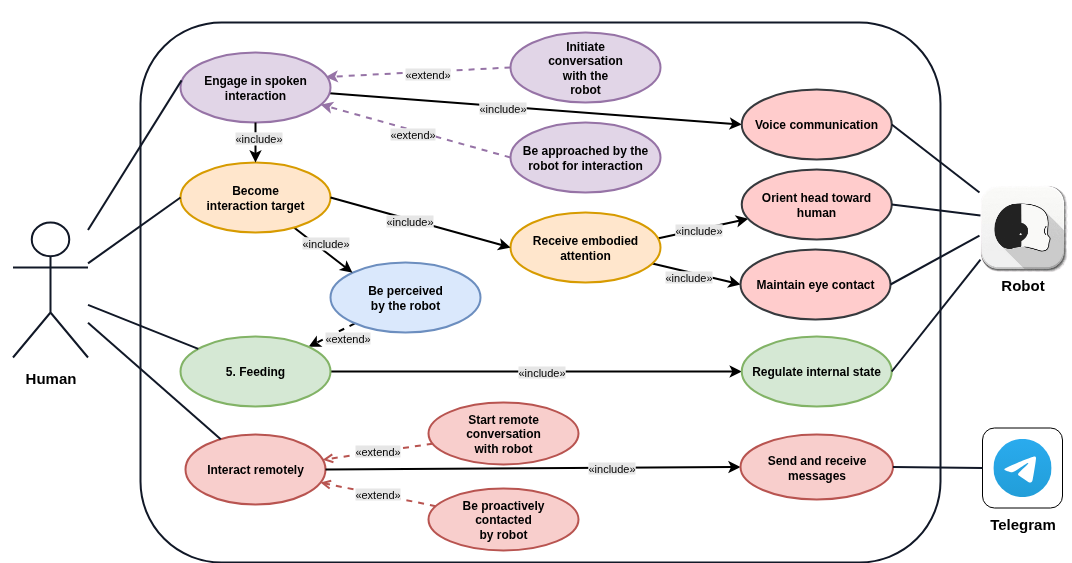
\includegraphics[width=0.88\textwidth,height=0.38\textheight,keepaspectratio]{Methodology/Figures/architecture-use-cases.png}
    \caption[Architecture use cases.]{Use-case diagram of the complete architecture, covering person perception, embodied attention, proactive and reactive spoken interaction, human-assisted internal-state regulation, and remote interaction through Telegram.}
    \label{fig:architecture-use-cases}
\end{figure}

\subsection{Stable transitions and proactive outreach}
\label{subsec:stable-transitions}

A remote state change takes effect only after it has held for $T_d=60$~s:

\begin{equation}
    \hat h(t)=h \quad\text{only if}\quad h_{\mathrm{eff}}(\tau)=h \quad\forall\tau\in[t-T_d,t].
    \label{eq:stable-remote-state}
\end{equation}

Subscribers are ranked by priority $P_u$, the learned affinity $A_{i(u)}$ of the person linked to account $u$, trusted only once that person has $n_{i(u)}\geq3$ recorded interactions:

\begin{equation}
    P_u=
    \begin{cases}
        A_{i(u)}, & n_{i(u)}\geq3,\\
        \varnothing, & n_{i(u)}<3\ \text{or unresolved}.
    \end{cases}
    \label{eq:remote-priority}
\end{equation}

In Hungry, the system contacts up to five subscribers with $P_u > 0.20$; in Starving, it sends its urgent request to all subscribers.

\section{Experimental design and procedure}
\label{sec:experimental-design}

\subsection{Study design and deployment}
\label{subsec:study-design-deployment}

The architecture was evaluated during an eight-day naturalistic deployment in the main office of the IIT CONTACT unit in Genova, on an iCub Halfie (Figure~\ref{fig:experimental-setup}). On each deployment day the always-on and behaviour architectures ran together online from 10:00 to 16:00. Phase~1 (4 days) assigned participants roles, so that the robot would meet both people who fed it and people who did not. Phase~2 (4 days) removed the roles. RQ1 to RQ3 are evaluated across both phases, with Phase~2 testing whether each effect held once nobody was following instructions; RQ4 rests on a questionnaire completed after Phase~2. Every controller constant was fixed before deployment, and the thresholds, meal sizes, action costs and affinity parameters used in the analysis were checked against the controller source code. Most were derived from the session length and the drain rate instead of being tuned to data; Appendix~\ref{app:constants} gives the reasoning behind each. The remote channel did change once: Telegram notices on entry into Hungry were first sent on 18 June 2026, the day six Telegram templates were reworded to address one recipient privately (Appendix~\ref{app:prompts}).

Two classical criteria frame the evaluation. Monitoring the resource and restoring it through feeding test whether homeostatic feedback works \citep{Cannon1929Homeostasis}. Deficit-conditioned action and affinity-dependent eligibility test whether internal state modulates how ready the robot is to act \citep{Tinbergen1951Instinct}. Agreement between the logged resource dynamics and the programmed ones verifies that the controller ran as specified. Behavioural success is judged only from observed consequences; for recovery, that means a logged rise in $x$.

\begin{figure}[tbp]
    \centering
    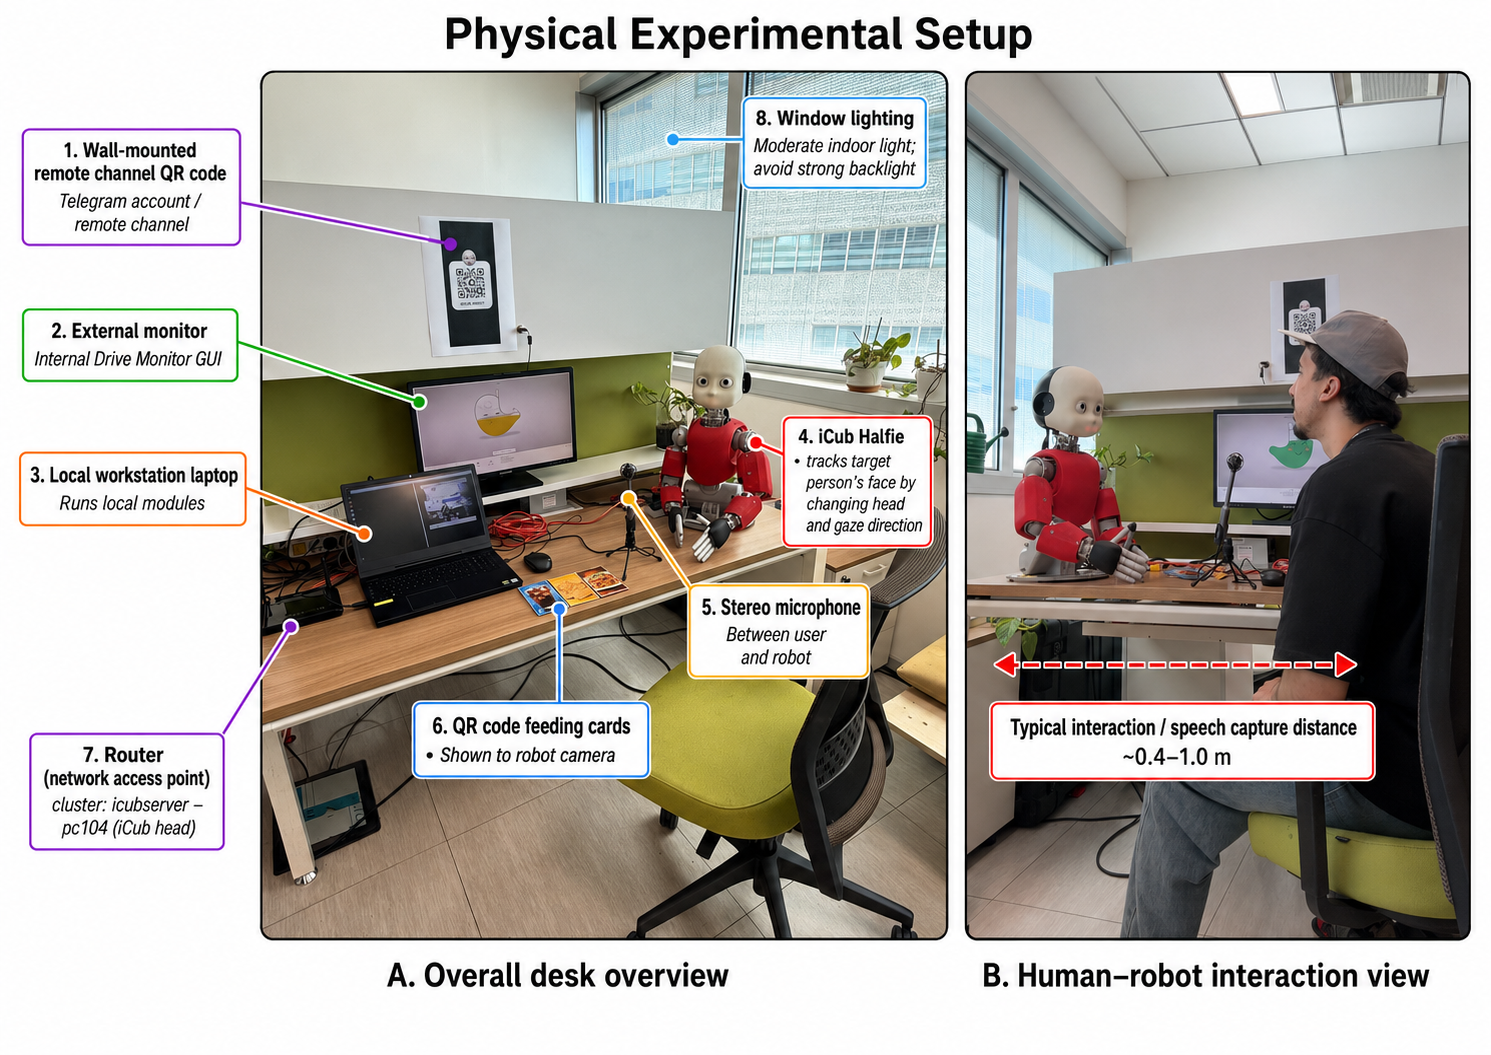
\includegraphics[width=0.88\textwidth,height=0.38\textheight,keepaspectratio]{Methodology/Figures/experimental-setup.png}
    \caption[Physical experimental setup.]{Physical experimental setup. Panel A identifies the remote-channel code, Internal Drive Monitor, local workstation, iCub Halfie, stereo microphone, feeding cards, network access point and window lighting. Panel B shows a typical interaction geometry and the speech-capture distance of about 0.4--1.0~m.}
    \label{fig:experimental-setup}
\end{figure}

\subsection{Participants and role conditions}
\label{subsec:participants-role-conditions}

Twelve adult participants enrolled (pseudonymised for analysis). Phase~1 assigned three roles by availability, not at random: Providers ($N=2$, instructed to feed frequently and respond promptly to remote alerts), Normal ($N=8$, unconstrained voluntary interaction), and Non-Providers ($N=2$, active daily interaction but prohibited from feeding). Phase~2 lifted these instructions without changing the cohort. All twelve attended at least one Phase~1 day and eleven attended at least one Phase~2 day, so every Phase~2 participant brought a Phase~1 role with them. Participants fed the robot with the feeding cards or the Internal Drive Monitor touchscreen.

\subsection{Questionnaire instruments and ethics}
\label{subsec:questionnaire-instruments}

The pre-interaction questionnaire collected demographics and a baseline on the 14-item Negative Attitudes toward Robots Scale (NARS) \citep{Nomura2006NARS}. The post-interaction questionnaire, given to all twelve participants after Phase~2, combined 15 Godspeed semantic differentials (naturalness, animacy, likeability) \citep{Bartneck2009Godspeed}, 12 RoSAS word associations on a 9-point scale \citep{Carpinella2017RoSAS}, 4 custom 5-point Likert items (hunger naturalness, hunger genuineness, belonging to the environment and motivation to help) and 4 open-ended prompts (Appendix~\ref{app:questionnaires}). The running system stored named face crops, Telegram chat identifiers and message text, and derived user profiles containing names, preferences, personal updates, and conversational style. Analytical exports replaced participant identities with pseudonyms. The study was approved under IIT ethics protocol \texttt{IIT\_INT\_HRI\_rev02}, and participants gave informed consent under the GDPR.

\subsection{Statistical framework and inference}
\label{subsec:statistical-framework}

Each outcome is counted in the unit that was directly observed: interactions for feeding and social-state outcomes, feeding events for meal choice, Starving episodes (reconstructed from the logged level) for recovery, hunger pings for remote replies, and logged target-selection records for the expression of affinity. Variation is inspected across phases and by leaving out one run or one named participant at a time. These ranges show how much any single run or person moves the result; they are not confidence intervals.

One exploratory model tests the deficit-to-feeding contrast: a Bayesian mixed-effects logistic regression. For interaction $j$ of an enrolled participant, the binary outcome $Y_j$ indicates whether at least one meal was received, and
\begin{equation}
\operatorname{logit}\!\left[P(Y_j=1)\right]
= \alpha + \beta_D D_j + \beta_P P_j + \beta_{DP}D_jP_j + u_{i[j]} + v_{r[j]},
\label{eq:feeding-glmm}
\end{equation}
where Table~\ref{tab:glmm-roles} defines each term and the identity and run intercepts are crossed.

\begin{table}[tbp]
    \centering
    \small
    \caption{Variables of the feeding model of Equation~\ref{eq:feeding-glmm}.}
    \label{tab:glmm-roles}
    \begin{tabular}{@{}>{\raggedright\arraybackslash}p{0.20\textwidth}>{\raggedright\arraybackslash}p{0.17\textwidth}>{\raggedright\arraybackslash}p{0.53\textwidth}@{}}
        \toprule
        \textbf{Role} & \textbf{Term} & \textbf{Meaning} \\
        \midrule
        Dependent variable & $Y_j$ & Whether interaction $j$ received at least one meal (1) or none (0). \\
        Fixed effect (independent variable) & $D_j$ & Deficit at interaction onset: Hungry or Starving (1) against Full (0). Hunger state arises from drain and action costs and was not assigned. \\
        Fixed effect (independent variable) & $P_j$ & Phase: Phase~2, with no roles (1), against Phase~1, with assigned roles (0). This is the one factor the design changed. \\
        Fixed effect (interaction) & $D_jP_j$ & Lets the deficit effect differ between phases. \\
        Fixed effect (baseline) & $\alpha$ & Log-odds of feeding for a Full interaction in Phase~1, for an average person on an average day. \\
        Random effect & $u_{i[j]}$ & Intercept for each participant: some people feed more readily than others, and one person contributes many interactions. \\
        Random effect & $v_{r[j]}$ & Intercept for each run (deployment day): staffing, duration and time of day differ between days. \\
        \bottomrule
    \end{tabular}
\end{table}

Pooling Hungry and Starving targets the regulatory contrast without a separate coefficient for the few Starving interactions. The model uses the interactions of the twelve enrolled participants: 23 interactions with unresolved identity and 14 belonging to two identities outside the roster are omitted. Role is left out of the model. The participant metadata fixed before analysis identifies only the two Providers and two Non-Providers, and the logs also contain identities outside the verified 12-person roster, so assigning all remaining identities to Normal would invent a design variable.

The model is estimated with Hamiltonian Monte Carlo using four chains, 2,000 warm-up iterations and 2,000 retained draws per chain. Fixed coefficients receive $\mathcal{N}(0,1.5)$ priors on the log-odds scale; identity and run standard deviations receive half-normal $\mathcal{N}^{+}(0,1)$ priors. Adjusted probabilities are posterior predictions standardised over the observed identities, runs and phase composition. Sampling was accepted only with $\hat R\leq1.01$, bulk effective sample size above 400 and no divergent transitions; posterior predictive totals were compared with the observed feeding count. These estimates describe an adjusted association within this deployment. Figure~\ref{fig:results-feeding-model} reports them, and Appendix~\ref{app:feeding-model} plots every fitted term.

Affinity effects on eligibility are recomputed exactly with the threshold rule of the deployed controller (Equation~\ref{eq:effective-interaction-threshold}). For every recorded candidate, the logged effective threshold is compared with the threshold the same social state would have at neutral affinity, with everything else held fixed.
Entries into Starving are counted from the moment the logged level falls below 25. Segments that were already below 25 when recording began are counted separately. A return to Full counts as recovery only when feeding produces it, not when an operator switches the drive on or off (a mode reset, which sets the reserve back to 100) or when observation simply ends. Meal choice is analysed by the state just before feeding, whereas feeding incidence uses the state at the start of the interaction. A Telegram message within 15 minutes of a hunger ping (a remote hunger notification) counts as a time-matched response. Each message goes to the most recent unanswered ping, each ping takes at most one message, and a recovery notification closes the preceding request window.
For RQ4, the respondent is the observation unit. The naturalness, animacy and likeability domains average items 1--5, 6--10 and 11--15 within each respondent; summaries report means and sample standard deviations, and Cronbach's $\alpha$ assesses their internal consistency. Permutation Wilcoxon signed-rank tests compare each domain with the neutral midpoint, with Holm correction across the three tests. The four custom items remain separate, with agreement defined as ratings of 4 or 5. Two-sided exact sign tests compare counts above and below the neutral midpoint of 3, omitting neutral ties and applying Holm correction across the four tests. An exploratory paired permutation Wilcoxon test contrasts helping motivation with perceived hunger naturalness; rank-biserial correlations report signed effect magnitude. Spearman correlations test whether baseline NARS scores track the three domains or the four custom outcomes. NARS measures general attitudes rather than a pre-test of the same perceptions. The $p$-values come from permutation, with Holm correction across seven correlations. Permutation procedures use 9,999 resamples with fixed random seeds. A sensitivity analysis excludes the respondent whose open response reports no interaction; otherwise open responses serve only to explain ratings. The RoSAS composites precomputed in the survey workbook are not validated factor scores, so the RoSAS word associations are reported item by item.
